% Kinematics
\section{Kinematics}
	
% Kinematics - Overview
\subsection{Overview}
		
Kinematics is the branch of mechanics that \textbf{describes} the motion of objects without necessarily discussing what causes the motion. We will learn to describe motion in three ways:
\begin{itemize}
	\item Using \textbf{words}
	\item Using \textbf{graphs}
	\item Using \textbf{equations}
\end{itemize}
	
% Kinematics - Particles
\subsection{Particles}
A particle is an object that has \textbf{mass} but \textbf{no volume}  and occupies a \textbf{position} described by \textbf{one point in space}. Physicists love to turn all objects into particles, because it makes the math  a lot easier.
	
% Kinematics - Distance (d)
\subsection{Distance (d)}
The total length of the path traveled by a particle is called \textbf{distance}. “How far have you walked?” is a typical distance question. The SI unit of distance is the meter.
	
% Kinematics - Displacement (\Deltax)
\subsection{Displacement ($\Delta x$)}
The change in the position of a particle is called \textbf{displacement}. $\Delta$ is a Greek letter used to represent the words “change in”. $\Delta x$ therefore means “change in x”. It is always calculated by final value minus initial value. “How far are you from home?” is a typical displacement question. The SI unit for displacement is the meter.
	
% Kinematics - Distance vs Displacement
\newpage
\subsection{Distance vs Displacement}
\begin{figure}[h]
	\centering
	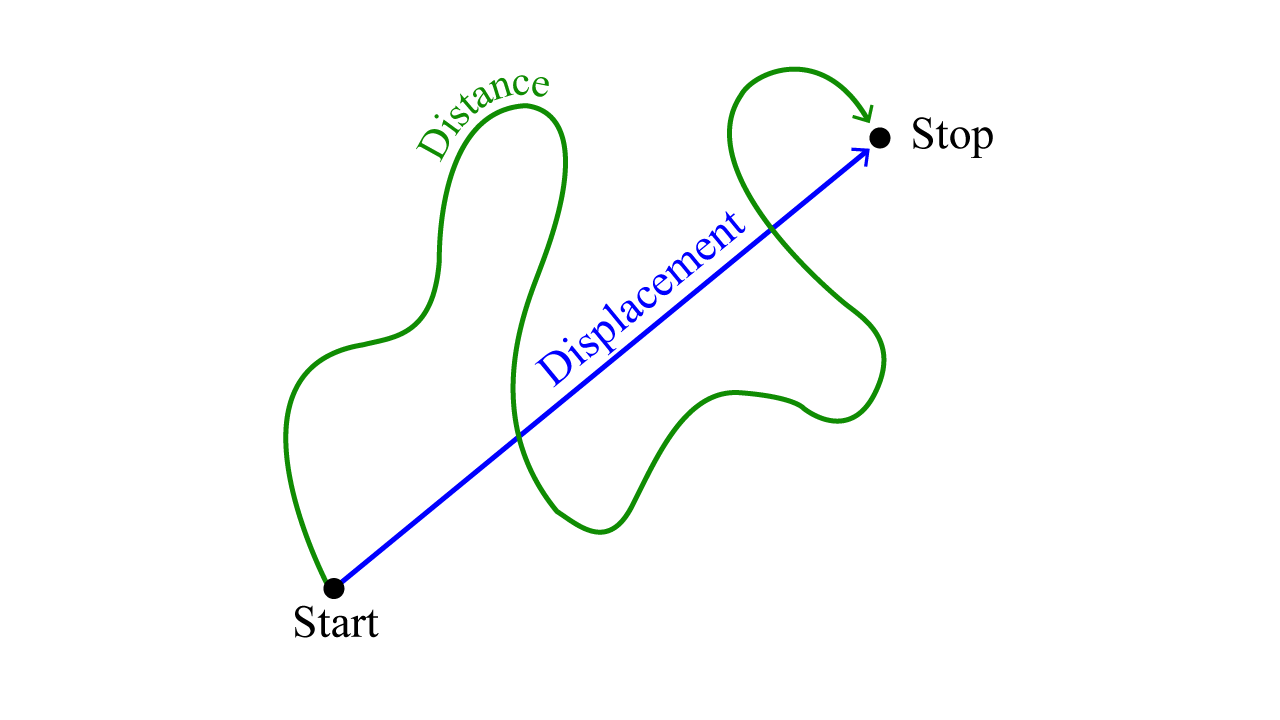
\includegraphics[scale=0.2]{images/distance-vs-displacementphoto}
	\caption{Distance vs Displacement Example}
	\label{fig:DisplacmentVsDistance}
\end{figure}
As seen above in figure \ref{fig:DisplacmentVsDistance}, a picture can help you distinguish between distance and displacement.